\chapter{Compact Models}
Here we introduce different formulations for the traveling salesman problem that we implemented. For all the following model we will use the decision variable $x_{ij}$ already defined in 1.2.

\section{Sequential formulation}
For this version, formulated by Miller, Tucker and Zemlin in 1960, we introduce the continuous variable 
\begin{equation*}
	u_i = \text{sequence in which point i is visited} \ (i \neq 1)
\end{equation*}
and the constraint 2.4. In total this formulation has $n^2-n+2$ constraints, $n(n-1)$ 0-1 variables and $(n-1)$ continuous variables.

\begin{subequations}
	\begin{equation}
		\text{min} \underbrace{\sum_{(i,j) \in A} c_{ij}x_{ij}}_\text{circuit cost}
	\end{equation}
	\begin{equation}
		\underbrace{\sum_{(i,j) \in \delta^{-}(j)} x_{ij} = 1}_\text{one edge incoming in j}, \quad j \in V 
	\end{equation}
	\begin{equation}
		\underbrace{\sum_{(i,j) \in \delta^{+}(j)} x_{ij} = 1}_\text{one edge outgoing in i}, \quad i \in V
	\end{equation}
	\begin{equation}
		u_i-u_j+nx_{ij} \leq n-1 \quad \forall i,j \in N-\lbrace 1 \rbrace, \ i\neq j
	\end{equation}
\end{subequations}

\section{Flow-based formulations}

\subsection{Single commodity flow}
Provided by Gavish and Graves in 1978, it adds continuous variables: 
\begin{equation*}
	y_{ij} = \text{flow in arch} \ (i,j) \ i \neq j
\end{equation*}
In total it has $n(n+2)$ constraints, $n(n-1)$ 0-1 variables and $n(n-1)$ continuous variables.
Note that the 2.2d can be improved substituting the second term with $(n-1)x_{ij}$

\begin{subequations}
	\begin{equation}
		\text{min} \sum_{(i,j) \in A} c_{ij}x_{ij} \\
	\end{equation}
	\begin{equation}
		\sum_{(i,j) \in \delta^{-}(j)} x_{ij} = 1, \quad j \in V \\
	\end{equation}
	\begin{equation}
		\sum_{(i,j) \in \delta^{+}(j)} x_{ij} = 1, \quad i \in V \\
	\end{equation}
	\begin{equation}
		y_{ij} \leq (n-1)x_{ij} \quad \forall i,j \in N, \ i \neq j \\
	\end{equation}
	\begin{equation}
		\sum_{j, \; j \neq 1} y_{1j} = n-1 \\
	\end{equation}
	\begin{equation}
		\sum_{i, \; i \neq j} y_{ij} - \sum_{k, \; i \neq k} y_{jk} = 1 \quad \forall j \in N - \lbrace 1 \rbrace
	\end{equation}
\end{subequations}

\subsection{Two commodity flow}
Created by Finke, Claus and Gunn in 1983. It maintains constraint 2.1b and 2.1c (from this point they and the objective function will not be shown in the formulation) and introduce the continuous variables:
\begin{equation*}
	y_{ij} = \text{flow of commodity 1 in arc} \ (i,j) \ i \neq j
\end{equation*}
\begin{equation*}
	z_{ij} = \text{flow of commodity 2 in arc} \ (i,j) \ i \neq j
\end{equation*}
and add the constraints:

\begin{subequations}
	\begin{equation}
	 	\sum_{j, \; j \neq 1} (y_{1j}-y_{j1}) = n-1
	\end{equation}
	\begin{equation}
		\sum_{j} (y_{ij}-y_{ji}) = 1 \quad \forall i \in N-\lbrace 1 \rbrace, \ i \neq j
	\end{equation}
	\begin{equation}
		\sum_{j, \; j \neq 1} (z_{1j}-z_{j1}) = -(n-1)
	\end{equation}
	\begin{equation}
		\sum_{j} (z_{ij}-z_{ji}) = -1 \quad \forall i \in N-\lbrace 1 \rbrace, \ i \neq j
	\end{equation}
	\begin{equation}
		\sum_{j} (y_{ij}+z_{ij}) = n-1 \quad \forall i \in N
	\end{equation}
	\begin{equation}
		y_{ij}+z_{ij} = (n-1)x_{ij} \quad \forall i, j \in N
	\end{equation}
\end{subequations}

In total it has $n(n+4)$ constraints, $n(n-1)$ 0-1 variables and $2n(n-1)$.

\subsection{Multi-commodity flow}
Proposed by Wong and Claus in 1984. Again constraint 2.1b and 2.1c are maintained. It introduce the continuous variable:
\begin{equation*}
	y_{ij}^k = \text{flow of commodity k in arc} \ (i,j) \in N-\lbrace 1 \rbrace
\end{equation*}
and the following constraints:
\begin{subequations}
	\begin{equation}
		y_{ij} \leq x_{ij} \quad \forall i,j,k \in N, \ k \neq 1
	\end{equation}
	\begin{equation}
		\sum_{i} y_{1i}^k = 1 \quad \forall k \in N-\lbrace 1 \rbrace
	\end{equation}
	\begin{equation}
		\sum_{i} y_{i1}^k = 0 \quad \forall k \in N-\lbrace 1 \rbrace
	\end{equation}
	\begin{equation}
		\sum_{i} y_{ik}^k = 1 \quad \forall k \in N-\lbrace 1 \rbrace
	\end{equation}
	\begin{equation}
		\sum_{j} y_{kj}^k = 0 \quad \forall k \in N-\lbrace 1 \rbrace
	\end{equation}
	\begin{equation}
		\sum_{i} y_{ij}^k - \sum_{i} y_{ji}^k = 0 \quad \forall j,k \in N-\lbrace 1 \rbrace, \ j \neq k
	\end{equation}
\end{subequations}
In total there are $n^3+n^2+6n-3$ constraints, $n(n-1)$ 0-1 variables and $n(n-1)^2$

\section{Time staged formulations}

\subsection{First stage dependent}
Introduced by Fox, Gavish and Graves in 1980. Constraint 2.1b and 2.1c are maintained, in addition we have 0-1 integer variables:
\[ y_{ij}^t =
	\begin{cases}
		1 \quad \text{if the edge} \ (i,j) \ \text{is traversed at stage t} \\
		0 \quad \text{otherwise}
	\end{cases}
\]
and constraints below, for a total of $n(n+2)$ constraints and $n(n-1)(n+1)$ 0-1 variables.

\begin{subequations}
	\begin{equation}
		\sum_{i,j,t} y_{ij}^t = n
	\end{equation}
	\begin{equation}
		\sum_{j,t \; t \geq 2} ty_{ij}^t - \sum_{k,t} ty_{ki}^t = 1 \quad \forall i \in N-\lbrace 1 \rbrace 
	\end{equation}
	\begin{equation}
		x_{ij}-\sum_{t} x_{ij}^t = 0 \quad \forall i,j \in N, \ i \neq j
	\end{equation}
	with the condition
	\begin{equation}
		y_{il}^t = 0 \; \forall t \neq n, \quad y_{ij}^t = 0 \; \forall t \neq 1, \quad y_{ij}^l = 0 \; \forall i \neq 1, \quad i \neq j
	\end{equation}
\end{subequations}

\subsection{Second stage dependent}
Provided by Fox, Gavish and Graves in 1980. It uses the same variables of first stage and constraints 2.1b and 2.1c and it adds:

\begin{subequations} 
	\begin{equation}
		\sum_{i,t \; i \neq j} y_{ij}^t = 1 \quad \forall j \in N
	\end{equation}
	\begin{equation}
		\sum_{j,t \; j \neq i} y_{ij}^t = 1 \quad \forall i \in N
	\end{equation}
	\begin{equation}
		\sum_{i \; j \neq i} y_{ij}^t = 1 \quad \forall t \in N
	\end{equation}
	\begin{equation}
		\sum_{j,t \; t \geq 2} ty_{ij}^t - \sum_{k,t} ty_{ki}^t = 1 \quad \forall i \in N-\lbrace 1 \rbrace
	\end{equation}
\end{subequations}
In totals there are $4n-1$ constraints and $n(n-1)(n+1)$ 0-1 variables.

\subsection{Third stage dependent}
Again we have the same variables of first stage and constraints 2.1b and 2.1c. In addition, 
for a total of $2n^2-n+3$ constraints and $n(n-1)(n+1)$ 0-1 variables we have:
\begin{subequations}
	\begin{equation}
		\sum_{j} y_{1j}^1 = 1
	\end{equation}
	\begin{equation}
		\sum_{i} y_{i1}^n = 1
	\end{equation}
	\begin{equation}
		\sum_{j} y_{ij}^t - \sum_{k} y_{ki}^{t-1} = 0 \quad \forall i,t \in N-\lbrace 1 \rbrace
	\end{equation}
\end{subequations}

\section{Final comparison between Compact Models}

\begin{figure}[H]
\centering
	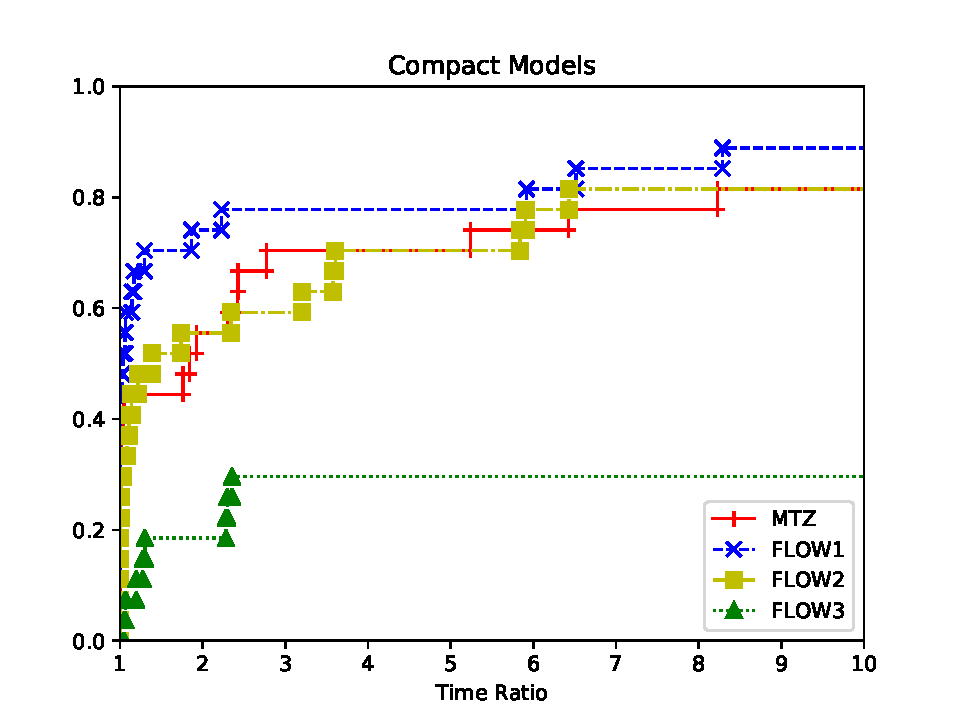
\includegraphics[scale=0.9]{media/compact10.pdf} \\
	\caption{Performance profile for compact models with time ratio 10}
	\label{fig:compacts10}
\end{figure}

\begin{figure}[H]
\centering
	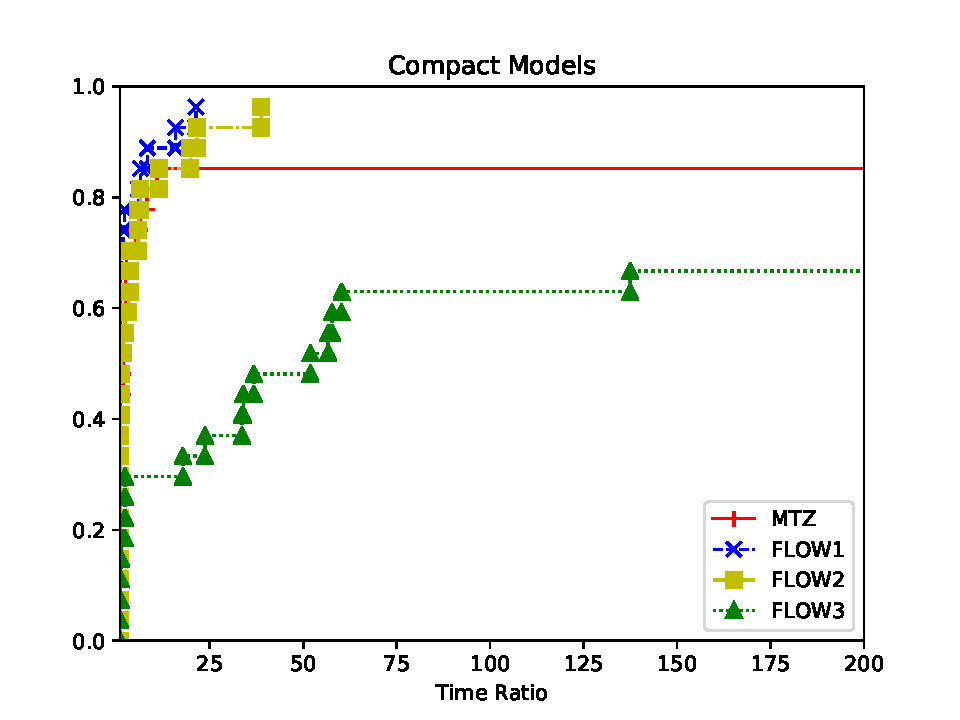
\includegraphics[scale=0.9]{media/compact200.pdf} \\
	\caption{Performance profile for compact models with time ratio 200}
	\label{fig:compacts200}
\end{figure}

We have decided to test the performance only for the MTZ's formulation and the Flow Based formulations. The main reason about this choice is the amount of time that is required for the Time staged formulations.
From the performance profile, it is possible to observe that the model that works best in practice is  the "Single Commodity Flow" one. Also the "Two Commodity Flow" and MTZ models obtained a decent score, while the "Multi Commodity Flow" was not so good. \\
The scope of Figure ~\ref{fig:compacts200} is to highlight the difference in performance between the "Multi Commodity Flow" model and the other ones.\\
As a remark, for the tests we used small datasets, with a number of nodes up to 80. Testing these compact models on bigger datasets would have been unfeasible for time reasons.

